\newpage 
\small 
\section*{Question 10}
\textbf{When the stock market crashes, what influenc does it have on investment, consumption, and aggregate demand? Why? 
How should the Federal Reserve respond? Why?}


A stock market crash lowers the market value of the capital that firms have already installed, which in turn reduces Tobin's q. 

When q<1, firms see that replacing or adding new capital isn’t profitable because the market value is below the cost of replacement. This discourages business investment. In addition, falling housing prices may reduce residential investment, and firms expecting lower future sales might cut back on inventory investment.

The crash also diminishes household wealth, especially for those holding stocks. This “wealth effect” erodes consumer confidence, causing households to scale back on discretionary spending. As consumption falls along with investment, aggregate demand drops significantly, shifting the AD curve to the left. The new equilibrium features lower output (Y) and a lower price level (P), which can lead to higher unemployment.

To offset the decline in aggregate demand, the Federal Reserve should adopt expansionary monetary policies. This might include lowering interest rates to make borrowing more affordable for businesses and consumers, thereby encouraging spending and investment. The Fed could also implement quantitative easing (QE) by purchasing long-term securities to inject liquidity into the financial system. Moreover, using forward guidance to commit to low interest rates for an extended period can further boost confidence and spending.

\begin{center}
    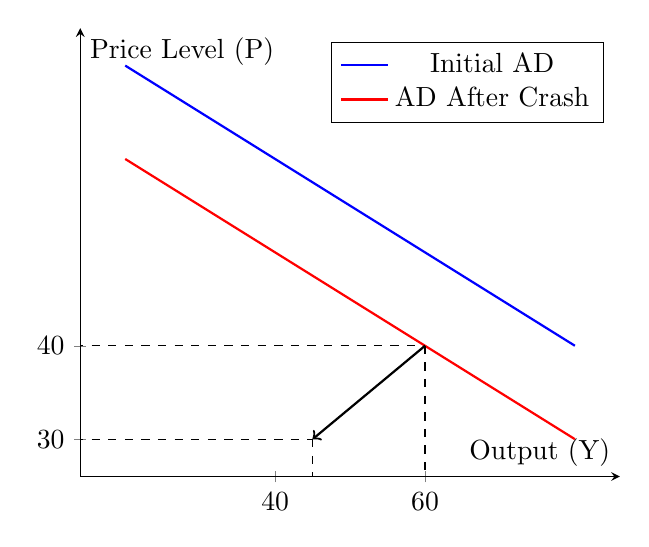
\begin{tikzpicture}
        \begin{axis}[
            axis lines = middle,
            xlabel = {Output (Y)},
            ylabel = {Price Level (P)},
            xtick={40, 60},
            ytick={30, 40},
            legend pos = north east,
            enlargelimits=true
        ]
            % Initial AD Curve
            \addplot[blue, thick, domain=20:80, samples=100] {80 - 0.5*x};
            \addlegendentry{Initial AD}
            
            % AD After Crash (shift left)
            \addplot[red, thick, domain=20:80, samples=100] {70 - 0.5*x};
            \addlegendentry{AD After Crash}

            % Equilibrium before crash
            \draw[dashed] (axis cs:60,40) -- (axis cs:60,0);
            \draw[dashed] (axis cs:0,40) -- (axis cs:60,40);
            \node[anchor=north] at (axis cs:60,0) {\small $Y_1$};
            \node[anchor=east] at (axis cs:0,40) {\small $P_1$};

            % Equilibrium after crash
            \draw[dashed] (axis cs:45,30) -- (axis cs:45,0);
            \draw[dashed] (axis cs:0,30) -- (axis cs:45,30);
            \node[anchor=north] at (axis cs:45,0) {\small $Y_2$};
            \node[anchor=east] at (axis cs:0,30) {\small $P_2$};

            % Arrow showing shift
            \draw[->, thick] (axis cs:60,40) -- (axis cs:45,30);
        \end{axis}
    \end{tikzpicture}
\end{center}

\section*{Question 11}
\textbf{It is an election year, and the eceonomy is in a recessio. The opposition candidate 
campaigns on a platform of passing an investment tax credit, which would be effective next year
after he takes office. What impact does this campaign promise have on economic conditions during the current year.} 

In an election year, when an opposition candidate promises to implement an investment tax credit (ITC) starting next year, it can significantly affect the economy in the current year. If firms believe the candidate will win and that the ITC will lower future capital costs, they may delay current investments, preferring to wait for the improved conditions. This postponement reduces investment spending, which in turn decreases aggregate demand.

The drop in investment can worsen a recession by lowering economic activity, raising unemployment, and further undermining consumer confidence. As the economy settles at a new equilibrium with lower output and price levels, the deepening recession may increase voter dissatisfaction with the incumbent, further boosting the opposition candidate's chances—a feedback loop that amplifies the downturn.

Additionally, uncertainty about the election and potential policy changes may lead households to cut back on spending, compounding the reduction in aggregate demand. To counter these effects, the incumbent government could introduce immediate fiscal stimulus—such as temporary tax cuts or increased government spending—to bolster economic activity. By providing policy stability and clear assurances that current measures will remain in place, the government can reduce uncertainty and encourage both investment and consumption, potentially offsetting the negative impact of delayed investments
\begin{center}
    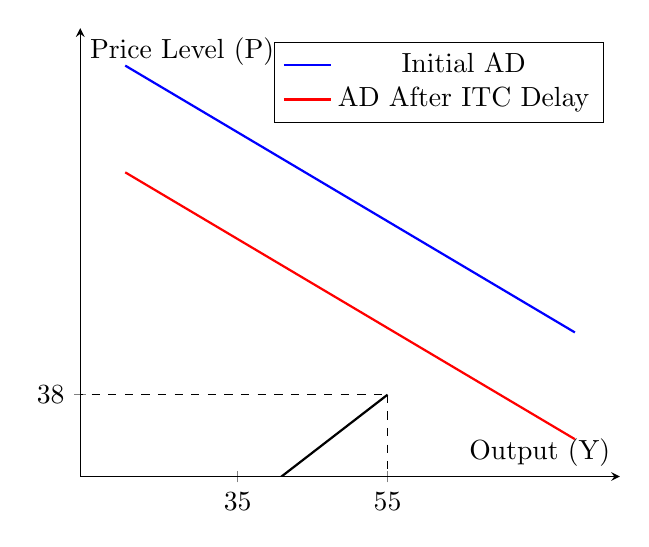
\begin{tikzpicture}
        \begin{axis}[
            axis lines = middle,
            xlabel = {Output (Y)},
            ylabel = {Price Level (P)},
            xtick={35, 55},
            ytick={25, 38},
            legend pos = north east,
            enlargelimits=true
        ]
            % Initial AD Curve
            \addplot[blue, thick, domain=20:80, samples=100] {85 - 0.5*x};
            \addlegendentry{Initial AD}

            % AD Shift Due to ITC Delay (leftward)
            \addplot[red, thick, domain=20:80, samples=100] {73 - 0.5*x};
            \addlegendentry{AD After ITC Delay}

            % Equilibrium before tax credit
            \draw[dashed] (axis cs:55,38) -- (axis cs:55,0);
            \draw[dashed] (axis cs:0,38) -- (axis cs:55,38);
            \node[anchor=north] at (axis cs:55,0) {\small $Y_1$};
            \node[anchor=east] at (axis cs:0,38) {\small $P_1$};

            % Equilibrium after tax credit delay
            \draw[dashed] (axis cs:35,25) -- (axis cs:35,0);
            \draw[dashed] (axis cs:0,25) -- (axis cs:35,25);
            \node[anchor=north] at (axis cs:35,0) {\small $Y_2$};
            \node[anchor=east] at (axis cs:0,25) {\small $P_2$};

            % Arrow showing shift
            \draw[->, thick] (axis cs:55,38) -- (axis cs:35,25);
        \end{axis}
    \end{tikzpicture}
\end{center}
